\section{Language Modeling with n-gram \& RNN}

\textbf{Goal}: Model the distribution over all finite sequences from $V^*$, where $V$ is the vocabulary set. The instance space is infinite.

\subsection*{Local Normalization}

Def: the sum of the probability of all children given their parents is 1. This guarantees the normalizer is 1.

Necessary Condition: every node has ``EOS'' as descendant (could be child or grandchild, etc.), o.w. there is a possible sequence of infinite length.

Sufficient Condition: every node $x$ has ``EOS'' as a child and $P(\text{EOS}\mid \text{x})\ge c$ for some positive constant $c$.

\subsection*{n-gram Assumption}

n-gram simplifies the problem by assuming each word only depends on the previous $n-1$ words, i.e.,
$p(y_t\mid y_{<t}) := p(y_t\mid y_{t-(n-1):t-1}) := \frac{\exp(w_{y_t}\cdot h_t)}{\sum_{y^\prime} \exp(w_{y^\prime}\cdot h_t)}$, where $w_y\in R^d$ is the word vector and $h_t$ is the n-gram context vector which encodes the previous $n-1$ words. ``BOS'' is padded for some $t<n$. $h_t:=f(y_{t-1}, \dots, y_{t-(n-1)})$ is computed by a neural network.

\subsection*{Recurrent Neural Network}

Change $h_t:=f(h_{t-1}, y_{t-1})$, where $f$ is still a neural network. This allows information from arbitrary distance.

\begin{enumerate}
    \item Vanilla RNN: $h_t=\sigma(W_1 h_{t-1}+W_2 e(y_{t-1}))$, $\sigma=\tanh$.
    \item LSTM: has a short-term memory $h_t$ and long-term memory $c_t$.
    \item GRU: a fix to the vanishing/exploding gradients.
\end{enumerate}
% \begin{center}
%     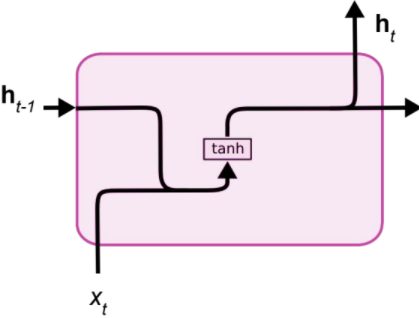
\includegraphics[width=.1\textwidth]{img/vanilla-RNN.png}
%     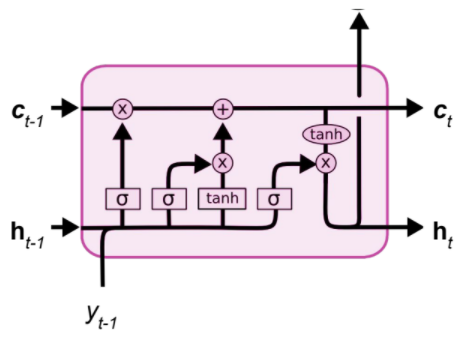
\includegraphics[width=.1\textwidth]{img/LSTM.png}
%     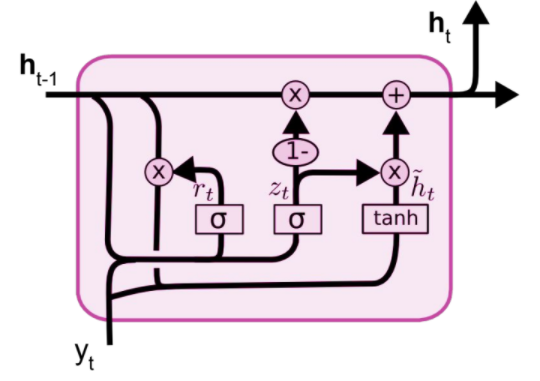
\includegraphics[width=.1\textwidth]{img/GRU.png}
% \end{center}
